\documentclass[10pt,twocolumn]{article}
\usepackage[letterpaper,margin=0.72in]{geometry}
\usepackage{amsmath,amssymb,siunitx,graphicx,booktabs,hyperref,authblk,microtype,xcolor}
\hypersetup{colorlinks=true,linkcolor=blue,citecolor=blue,urlcolor=blue}
\sisetup{detect-all}
\setlength{\columnsep}{0.25in}
\title{\bfseries Aperture-Dependent Acoustic Modes and Photoelastic Overlap in a Suspended Three-Dimensional Lithium-Niobate IDT Structure}
\author[1]{[Author name(s) to be completed]}
\affil[1]{[Affiliation(s) to be completed]}
\date{\small Draft for internal review --- fabrication and experimental validation pending}
\begin{document}
\twocolumn[\maketitle
\begin{center}\fbox{\parbox{0.94\textwidth}{\centering\small\color{red!70!black}
\textbf{PREPRINT DRAFT.} This manuscript reports numerical eigenmode and post-processed overlap calculations only. The proposed device has not yet been fabricated or experimentally characterized. All fabrication and measurement fields marked ``pending'' must be completed before public preprint release.}}\end{center}
\begin{abstract}
Suspended thin-film lithium niobate (TFLN) acoustic structures offer a route to compact gigahertz acousto-optic devices, but the finite aperture of an interdigital-transducer (IDT) region can alter both the acoustic spectrum and the spatial distribution of optical--acoustic overlap. Here, we numerically compare the eigenmodes of a suspended three-dimensional IDT structure over aperture lengths from 4 to \SI{16}{\micro\meter}. For each geometry, twelve eigenmodes near \SI{3.33}{\giga\hertz} are computed in COMSOL Multiphysics 6.3. We post-process the exported strain fields using a photoelastic perturbation model for an optical field propagating along the acoustic periodic direction, and evaluate a Gaussian optical intensity profile across the aperture. Within a \SIrange{3.28}{3.38}{\giga\hertz} target band, a \SI{6}{\micro\meter} aperture supports a candidate mode at \SI{3.304}{\giga\hertz} with an interior overlap proxy of \SI{39.54}{\joule^{-1/2}} for a \SI{1}{\micro\meter} optical intensity full width at half maximum (FWHM). In the same mode, the largest edge-band value is \SI{66.77}{\joule^{-1/2}}, indicating that optical placement near the electrode ends can dominate the interior value. A preliminary mesh-refinement audit changes the selected modes and the aperture ranking: for the \SI{10}{\micro\meter} geometry, the best target-band overlap proxy rises from \SI{34.05}{\joule^{-1/2}} on the baseline mesh to \SI{111.82}{\joule^{-1/2}} on the refined mesh, but the refined candidate does not match the baseline mode shape. The \SI{6}{\micro\meter} candidate is more consistent in overlap magnitude, yet its most similar refined mode shifts by about \SI{12.9}{\mega\hertz}. Thus the current sweep identifies a promising \SI{3.3}{\giga\hertz} design region but does not establish a mesh-converged aperture optimum. A separate exploratory 1 V coupled electromechanical calculation shows a mode-projected response peak at \SI{3.3057}{\giga\hertz} on one mesh. A single-pole fit gives a preliminary simulated FWHM of \SI{1.13}{\mega\hertz} ($Q\approx2.9\times10^3$) under an assumed structural loss factor; this value is not measured or mesh-validated. A first-order photoelastic-only effective-index perturbation per volt is estimated using an assumed slab-mode/Gaussian optical weighting, but the actual waveguide mode, moving-boundary contribution, modulation efficiency, and measured device performance remain unevaluated; fabrication and experimental validation are pending.
\end{abstract}
\noindent\textbf{Keywords:} thin-film lithium niobate; suspended acoustic resonator; interdigital transducer; photoelastic overlap; aperture optimization; acousto-optics\vspace{1em}]
\section{Introduction}
Integrated acousto-optic (AO) devices use acoustic waves to perturb an optical mode through photoelasticity, moving-boundary effects, or both. Lithium niobate is attractive because it combines strong piezoelectricity with a useful optical transparency window. GHz AO modulation has been demonstrated on thin-film lithium-niobate platforms, including waveguide-based implementations \cite{Cai2019,Yu2021,Chen2021}. Those demonstrations motivate designs that co-localize optical and acoustic fields while keeping the acoustic mode in a useful frequency range.

For a finite suspended IDT structure, the aperture is a consequential design variable: it changes the available interior region, the mode spectrum, and the spatial pattern sampled by an optical waveguide. A mode with a large global strain amplitude need not provide the largest overlap at a manufacturable waveguide position. Edge-localized overlap can also exceed the value in the nominal interior, which matters when the optical guide must be placed away from electrode tips.

This study provides a numerical aperture sweep for one suspended 3D TFLN/Al geometry. We use a photoelastic overlap proxy to compare candidate modes and optical positions, then identify a \SI{6}{\micro\meter} aperture as a candidate near \SI{3.3}{\giga\hertz}. The analysis is intended for design screening. The reported overlap proxy is not a driven electromechanical response or an experimentally measured AO efficiency.
\section{Device geometry and numerical methods}
\subsection{Suspended IDT model}
The simulated structure comprises a \SI{500}{\nano\meter}-thick suspended lithium-niobate slab with \SI{100}{\nano\meter}-thick aluminum electrodes. The acoustic periodicity is fixed at $p=\SI{2.58}{\micro\meter}$, with electrode duty cycle 0.25. The periodic direction is $x$; the finite aperture extends along $z$. The electrode region begins at $z_0=\SI{2}{\micro\meter}$, and the modeled stack includes a \SI{2}{\micro\meter} margin beyond each electrode end. The aperture length $W_{\mathrm{ap}}$ is swept over 4, 4.5, 4.75, 5, 5.25, 5.5, 6, 8, 10, 12, 14, and \SI{16}{\micro\meter}.

For every aperture, the geometry and mesh are rebuilt and twelve eigenmodes are solved around a \SI{3.33}{\giga\hertz} shift using COMSOL Multiphysics 6.3. The exported eigenfields include displacement, strain, and strain-energy density. The \SI{10}{\micro\meter} case is included as a reference configuration. Mode indices are solver ordering within each geometry; they are not assumed to identify the same physical branch across different apertures.
\subsection{Optical weighting and photoelastic proxy}
The optical field is assumed to propagate along $x$, parallel to the acoustic periodic direction. At a wavelength of \SI{1.55}{\micro\meter}, the optical weighting across the slab thickness uses a fundamental slab-mode intensity profile for TE or TM polarization. The calculation uses $n_e=2.138$, $n_o=2.211$, and the photoelastic coefficients $p_{11}=-0.026$, $p_{12}=0.090$, $p_{13}=0.133$, $p_{31}=0.179$, and $p_{33}=0.071$ as implemented in the analysis script.

The strain-induced refractive-index perturbation is constructed from the corresponding polarization-dependent photoelastic tensor contraction. The field is averaged over one acoustic period along $x$, weighted by the slab-mode intensity along $y$, then convolved across $z$ with a Gaussian optical intensity window. The Gaussian is parameterized by FWHM values of 0.5, 1.0, and \SI{1.5}{\micro\meter}. For the recommendation analysis, we use TE polarization and a \SI{1}{\micro\meter} FWHM.

To compare mode shapes independently of arbitrary eigenvector amplitude, the overlap is normalized by the square root of the integrated strain energy in lithium niobate, $U_{\mathrm{LN}}$:
\begin{equation}
g_{\mathrm{proxy}}(z_c)=\frac{\left|\int \Delta n_{\mathrm{PE}}(x,y,z)W_{\mathrm{opt}}(y,z;z_c)\,dV\right|}{\sqrt{U_{\mathrm{LN}}}\,\mathcal{N}(z_c)},
\end{equation}
where $z_c$ is the optical-guide center and $\mathcal{N}$ normalizes the optical weighting. Under this normalization, the quantity is reported in $\mathrm{J}^{-1/2}$. It is an eigenfield overlap proxy; it is not a voltage-normalized coupling coefficient or a power-conversion efficiency.

The edge band is defined as the first \SI{1}{\micro\meter} from either electrode end. The interior region excludes the first and last \SI{2}{\micro\meter} of the electrode aperture. For each mode, we record the maximum proxy within the edge band and within the interior. The target-band recommendation retains TE modes between 3.28 and \SI{3.38}{\giga\hertz}.
\section{Results}
\subsection{Target-band candidate}
The \SI{6}{\micro\meter} aperture contains a target-band mode at \SI{3.304066}{\giga\hertz}. For this mode, the maximum interior proxy is \SI{39.54}{\joule^{-1/2}} at $z_c=\SI{5.5}{\micro\meter}$. The same mode reaches \SI{66.77}{\joule^{-1/2}} in the edge band at $z_c=\SI{7.7}{\micro\meter}$, giving an edge-to-interior ratio of 1.69. The result suggests that the optical guide should be placed in the interior if the objective is to avoid an edge-dominated overlap profile; it does not mean that the edge is intrinsically undesirable for every device layout.

On the baseline mesh, the \SI{6}{\micro\meter} case provides the largest interior proxy among the tabulated target-band candidates. This ranking is provisional pending the mesh-refinement audit below. The \SI{4}{\micro\meter} aperture has no finite interior span under the chosen two-micrometer end margins; its tabulated interior value comes from a single sampled position and is included only for completeness, not treated as a practical design candidate. Its interior value is approximately 16\% greater than the \SI{10}{\micro\meter} reference (\SI{34.05}{\joule^{-1/2}} at \SI{3.302075}{\giga\hertz}). The edge-to-interior ratio is 1.69 for \SI{6}{\micro\meter} and 1.74 for \SI{10}{\micro\meter}. These modest ratio differences should not be interpreted as a robust advantage without mesh-convergence and fabrication-tolerance analysis.
\begin{figure}[t]\centering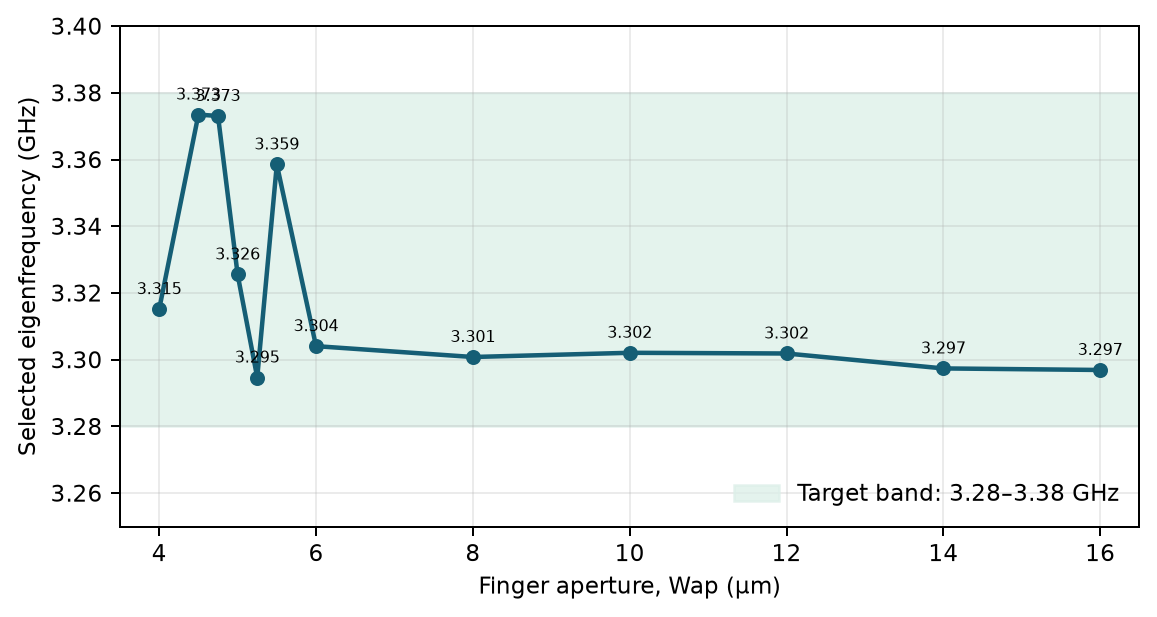
\includegraphics[width=\columnwidth]{images/frequency_vs_aperture.png}\caption{Baseline-mesh frequency of the target-band mode selected for each aperture by its interior overlap proxy. Shading indicates the \SIrange{3.28}{3.38}{\giga\hertz} selection range. Mode indices can change between geometries; plotted points are not branch tracking.}\label{fig:frequency}\end{figure}
\begin{figure}[t]\centering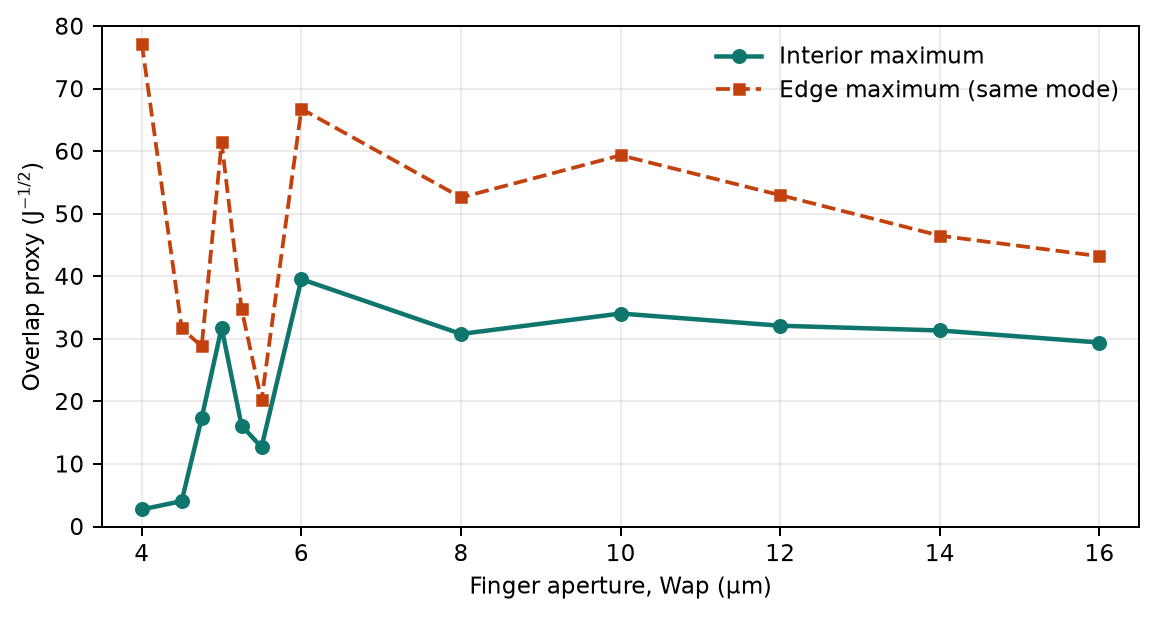
\includegraphics[width=\columnwidth]{images/overlap_vs_aperture.png}\caption{Baseline-mesh interior and same-mode edge maxima of the normalized photoelastic overlap proxy for the target-band candidate at each aperture.}\label{fig:overlap}\end{figure}
\subsection{Aperture and edge comparison}
Figure~\ref{fig:frequency} summarizes the frequency of the best interior-overlap target-band candidate at each aperture. The selection criterion is applied separately at each aperture; mode number alone is not used as a cross-geometry mode-tracking rule. Figure~\ref{fig:overlap} compares the interior maximum with the edge maximum of that same selected mode. Across most apertures, the edge proxy is larger than the interior proxy. This makes the optical position a design variable alongside aperture length.

The \SI{5}{\micro\meter} geometry has a different high-overlap mode outside the target band: a mode at \SI{3.423687}{\giga\hertz} reaches an interior proxy of \SI{140.73}{\joule^{-1/2}}. This mode is approximately \SI{94}{\mega\hertz} above \SI{3.33}{\giga\hertz}. It is therefore not selected for the stated target-band comparison, but may be a candidate if the intended operating frequency is moved upward and the branch is confirmed with a dedicated continuation study.
\begin{table*}[t]\centering\caption{Baseline-mesh target-band comparison for TE polarization and \SI{1}{\micro\meter} optical FWHM.}\label{tab:comparison}\begin{tabular}{@{}lcc@{}}\toprule
Quantity & $W_{\mathrm{ap}}=6$\,µm & $W_{\mathrm{ap}}=10$\,µm\\\midrule
Selected frequency (GHz) & 3.304066 & 3.302075\\
Interior $g_{\mathrm{proxy}}$ (J$^{-1/2}$) & 39.54 & 34.05\\
Interior position $z_c$ ($\si{\micro\meter}$) & 5.5 & 9.5\\
Same-mode edge maximum (J$^{-1/2}$) & 66.77 & 59.35\\
Edge/interior ratio & 1.69 & 1.74\\\bottomrule\end{tabular}\end{table*}
\section{Mesh-refinement and mode-tracking audit}
A second set of eigenmode simulations was run for $W_{\mathrm{ap}}=6$ and \SI{10}{\micro\meter} after tightening the mesh limits from $h_{\max}/h_{\min}=150/40$ nm (LN) and $80/20$ nm (Al) to $100/25$ nm (LN) and $50/12$ nm (Al). The target-band selection was repeated using the same photoelastic post-processing. These two mesh levels are an initial sensitivity audit, not a demonstrated asymptotic convergence study.

To compare mode shapes despite solver reordering, the effective TE photoelastic strain scalar was linearly interpolated on a shared spatial grid and its absolute normalized inner product was calculated between the baseline candidate and every refined mode. At $W_{\mathrm{ap}}=6$ the most similar refined field is mode 2 (correlation 0.915), at \SI{3.291194}{\giga\hertz}; its interior proxy is \SI{35.42}{\joule^{-1/2}}, about 10\% below the baseline value. At $W_{\mathrm{ap}}=10$, the highest shape correlation is only 0.420 (refined mode 6, \SI{3.291776}{\giga\hertz}), which is insufficient to claim a reliable one-to-one mode match. The refined-mesh target-band winner at 10 µm is mode 11 at \SI{3.364042}{\giga\hertz} with a much larger proxy, but its field correlation with the baseline winner is 0.219. This indicates that the apparent winner is sensitive to mesh and mode selection.

\begin{table}[t]\centering
\caption{Initial mesh audit for the two candidate apertures. Refined-mesh ``best'' rows maximize the interior proxy over all modes in the target band; matched rows use the maximum absolute normalized photoelastic-field correlation to the baseline winner.}
\label{tab:mesh-audit}
\begin{tabular}{@{}lcc@{}}\toprule
Quantity & 6 µm & 10 µm\\\midrule
Baseline winner $f$ (GHz) & 3.304066 & 3.302075\\
Baseline winner $g_{\mathrm{int}}$ (J$^{-1/2}$) & 39.54 & 34.05\\
Refined winner $f$ (GHz) & 3.311762 & 3.364042\\
Refined winner $g_{\mathrm{int}}$ (J$^{-1/2}$) & 42.70 & 111.82\\
Best-correlated refined mode & 2 & 6\\
Shape correlation & 0.915 & 0.420\\
Matched-mode refined $f$ (GHz) & 3.291194 & 3.291776\\
Matched-mode refined $g_{\mathrm{int}}$ (J$^{-1/2}$) & 35.42 & 38.18\\\bottomrule\end{tabular}\end{table}

The baseline sweep also selects $W_{\mathrm{ap}}=6$ µm as the TE interior-overlap maximum for optical intensity FWHM values of 0.5, 1.0, and 1.5 µm. The selected mode changes for the 1.5 µm spot, and this spot-size result has not yet been re-evaluated across the full aperture range on the refined mesh.

We also increased post-processing resolution from 130 by 25 samples per acoustic period/slab cross-section and 0.1 µm spacing along $z$ to 195 by 38 samples and 0.05 µm $z$ spacing for the baseline 6 and 10 µm candidates. The interior proxy changed by -0.02\% and +0.46\%, respectively; the edge maxima changed by +3.14\% and -5.82\%. Thus the post-processing grid is comparatively stable for these two modes, while the finite-element mesh and mode selection are not yet established as converged.

\section{Discussion}
The baseline aperture sweep identifies a candidate geometry near \SI{3.3}{\giga\hertz} under the stated optical and normalization assumptions. However, the two-level mesh audit changes the selected mode and, for the 10 µm case, the apparent aperture ranking. The 6 µm geometry remains a promising candidate, but its status as an optimum is unresolved until a finer multi-level convergence and mode-continuation study is completed. The overlap also depends on the assumed optical mode, photoelastic coefficients, eigenmode normalization, and exact waveguide placement. The aperture-overlap comparison remains an eigenmode-only analysis. A separate 6 µm coupled electromechanical model with a 1 V terminal drive and an assumed structural loss factor of $5\times10^{-4}$ produced nonzero displacement and strain. The volume-averaged components vary smoothly, but projection of the complex response onto the same-mesh 3.305664 GHz eigenvector shows a clear response maximum at that frequency. This projection is unweighted and normalized only relative to its peak; it establishes a simulated acoustic resonance in this model but not an absolute modal amplitude or measured Q. The 3.285--3.296 GHz sweep is an off-resonance background reference for this 100/50 nm model. A first-order photoelastic-only effective-index perturbation per volt was estimated with the assumed TE slab and Gaussian optical weighting: at 3.305664 GHz, $|\Delta n_{\rm eff}|=1.545\times10^{-7}$/V at the previously selected $z_c=5.5$ µm, with an interior maximum of $1.610\times10^{-7}$/V at 6.0 µm and an edge maximum of $1.266\times10^{-7}$/V at 7.0 µm. The edge/interior ratio is 0.786 for this driven mode, differing from the arbitrary-normalized eigenmode proxy. These estimates omit the actual waveguide optical eigenmode and moving-boundary term; they do not establish phase-modulation depth or sideband efficiency. The assumed loss factor is not measured, and the original aperture ranking remains provisional.

In the original arbitrary-normalized eigenmode proxy, edge maxima exceed the interior values for the selected 6 µm and 10 µm modes. The refined-mesh 10 µm winner instead has an interior maximum larger than its edge maximum, so this trend is mode- and mesh-dependent. The later 1 V driven calculation with assumed TE/Gaussian weighting also places the interior maximum above the edge maximum for that one 6 µm mode; neither comparison is yet based on the actual waveguide optical mode. Edge placement should therefore remain a geometry-dependent design choice pending the full optomechanical calculation.

Before treating the numerical ranking as final, the following checks remain: (i) complete a finer mesh and numerical extrapolation for the original photoelastic aperture sweep; (ii) repeat the full 12-aperture sweep on a refined mesh; (iii) check the crystallographic/photoelastic tensor orientation and material-parameter sensitivity; and (iv) repeat the mode-projected driven response on a second mesh with justified electrical and mechanical loading. The optical spot-width sweep is complete on the baseline mesh but still needs confirmation on the refined full sweep. The actual-mode optical perturbation including moving-boundary effects, a converged voltage-normalized response, and sideband efficiency also remain to be calculated. Measurements should then compare the fabricated resonance frequency, linewidth, RF-to-acoustic response, and optical modulation with the simulation.
\subsection{Exploratory coupled electromechanical check}
To test whether the candidate acoustic mode is excitable by the IDT, we added the piezoelectric charge-conservation equation to a separate 6 µm model and compared short-circuit coupled eigenmodes across four LN/Al mesh settings. The displacement-field MAC between successive tracked modes was 0.973, 0.994, and 0.995. The corresponding frequencies were 3.337995, 3.305664, 3.294186, and 3.290168 GHz. The final mesh refinement changed the tracked frequency by 0.122%, but the frequency continued to drift downward; this exploratory check does not establish a converged frequency or update the aperture ranking from the original eigenmode sweep.
\begin{table}[t]\centering\small
\caption{Tracked short-circuit coupled mode in one 6 µm model. MAC is an unweighted nearest-node displacement-field correlation to the next finer mesh.}
\label{tab:coupled-mesh}
\begin{tabular}{@{}rrrrr@{}}\toprule
LN/Al $h_{\max}$ (nm) & Mode & $f$ (GHz) & MAC & Change (\%)\\\midrule
150/80 & 4 & 3.337995 & 0.973 & ---\\
100/50 & 2 & 3.305664 & 0.994 & 0.969\\
75/38 & 2 & 3.294186 & 0.995 & 0.347\\
65/33 & 2 & 3.290168 & --- & 0.122\\\bottomrule
\end{tabular}\end{table}

A 1 V frequency-domain drive with the opposite terminal grounded returned nonzero fields. With an assumed structural loss factor of $5\times10^{-4}$, the component-wise LN volume averages of absolute displacement changed smoothly from 5.98, 1.23, and 5.60 pm at 3.285 GHz to 6.83, 1.34, and 6.01 pm at 3.296 GHz; this sweep is below the corresponding 100/50 nm coupled eigenmode and serves only as an off-resonance reference. A coarse sweep at 2 MHz spacing included the matching 3.305664 GHz eigenmode but did not resolve a clear peak in the volume averages. We therefore projected the complex displacement at five frequencies onto the corresponding same-mesh eigenvector over 46,647 LN nodes. The relative projection amplitudes at detunings $-1$, $-0.5$, $0$, $+0.5$, and $+1$ MHz are 0.480, 0.740, 1.000, 0.758, and 0.504, respectively, with a phase rotation through the center frequency. This mode-projected response has a clear maximum at the coupled eigenfrequency and confirms that the IDT excites the tracked mode in the simulated model. Additional projections at +2.336, +4.336, and +6.336 MHz decay to 0.250, 0.145, and 0.105 of the peak. A single-pole complex Lorentzian fit to the ten-point projection gives $f_0=3.305676$ GHz and FWHM $1.132$ MHz ($Q\approx2.92\times10^3$), with 1.02\% normalized RMS residual. This is a preliminary simulation result under the assumed loss factor $\eta_s=5\times10^{-4}$, not a measured or mesh-validated $Q$. The projection itself is unweighted and peak-normalized, so it does not give an absolute modal amplitude. The optical photoelastic and moving-boundary overlap, modulation index, and sideband efficiency remain unresolved.
\begin{figure*}[t]\centering
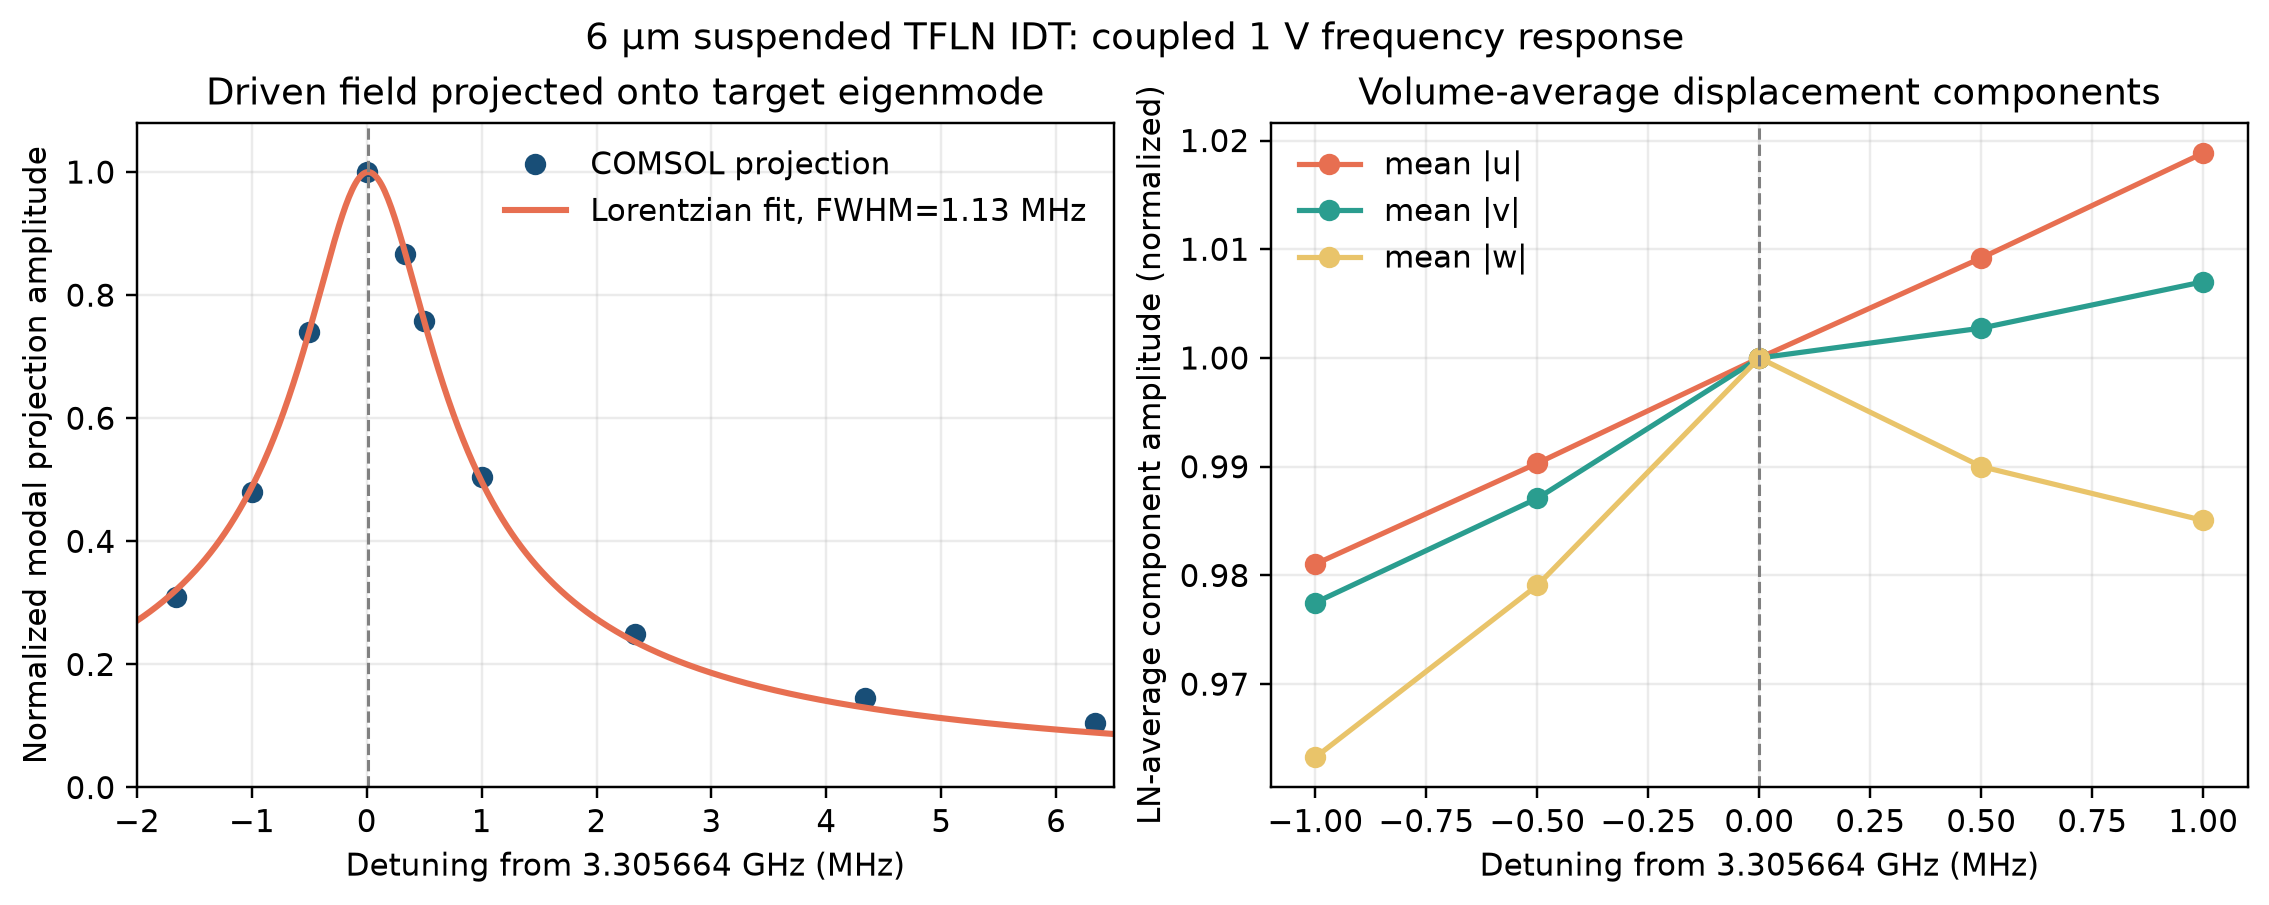
\includegraphics[width=0.96\textwidth]{images/coupled_drive_projection.png}
\caption{Exploratory 1 V response of the 6 µm coupled model on the 100/50 nm mesh. Left: complex displacement projected onto the matching 3.305664 GHz eigenvector, normalized to its peak magnitude. Right: LN volume-averaged absolute displacement components, normalized at the center frequency. The projected modal response shows a resonance peak that is not apparent in the volume averages. The nodal projection uses ten coarse and fine sweep points; its single-pole fit gives a preliminary FWHM of 1.13 MHz under assumed loss. The projection is unweighted and relative, not an absolute modal amplitude or measured Q.}
\label{fig:coupled-drive}
\end{figure*}

\begin{table*}[t]\centering\small
\caption{Five-point 1 V sweep around the matching 100/50 nm short-circuit mode. Displacement and strain columns are LN volume averages of absolute values; the assumed structural loss factor is $5\times10^{-4}$.}
\label{tab:drive-fine}
\begin{tabular}{@{}rrrrrr@{}}\toprule
$f$ (GHz) & $|u|$ (pm) & $|v|$ (pm) & $|w|$ (pm) & $|e_{xx}|$ & $|e_{xz}|$\\\midrule
3.304664 & 7.859 & 1.479 & 6.555 & $1.938\times10^{-5}$ & $1.622\times10^{-5}$\\
3.305164 & 7.933 & 1.494 & 6.663 & $1.958\times10^{-5}$ & $1.647\times10^{-5}$\\
3.305664 & 8.010 & 1.513 & 6.805 & $1.980\times10^{-5}$ & $1.681\times10^{-5}$\\
3.306164 & 8.084 & 1.518 & 6.737 & $1.995\times10^{-5}$ & $1.677\times10^{-5}$\\
3.306664 & 8.161 & 1.524 & 6.704 & $2.013\times10^{-5}$ & $1.683\times10^{-5}$\\\bottomrule
\end{tabular}\end{table*}

\subsection{First-order photoelastic perturbation per volt}
The driven strain fields were post-processed with the assumed scalar TE slab-mode intensity profile ($n_e=2.138$) and a 1 µm-FWHM Gaussian lateral optical weighting, matching the original screening model. At 3.305664 GHz, the photoelastic-only effective-index perturbation is $|\Delta n_{\rm eff}|=1.545\times10^{-7}$/V at $z_c=5.5$ µm. The maximum over the chosen interior band (4--6 µm) is $1.610\times10^{-7}$/V at 6.0 µm. The edge-band maximum (2--3 and 7--8 µm) is $1.266\times10^{-7}$/V at 7.0 µm, so the edge/interior ratio is 0.786 for this driven mode. The phase perturbation at 5.5 µm is $6.26\times10^{-4}$ rad mm$^{-1}$ V$^{-1}$. This driven, voltage-normalized comparison places the interior maximum above the edge maximum, unlike the original arbitrary-normalized eigenmode proxy. It applies only to this one mesh, assumed optical weighting, and assumed loss model.

This is a first-order photoelastic-only estimate, not a full optical eigenmode perturbation calculation. It omits the actual waveguide optical field, moving-boundary effects, and optical-mode normalization; it cannot by itself establish modulation depth or sideband conversion efficiency. The frequency-dependent profiles and edge/interior comparison are shown in Fig.~\ref{fig:drive-pe} and supplied as CSV data.
\begin{figure}[t]\centering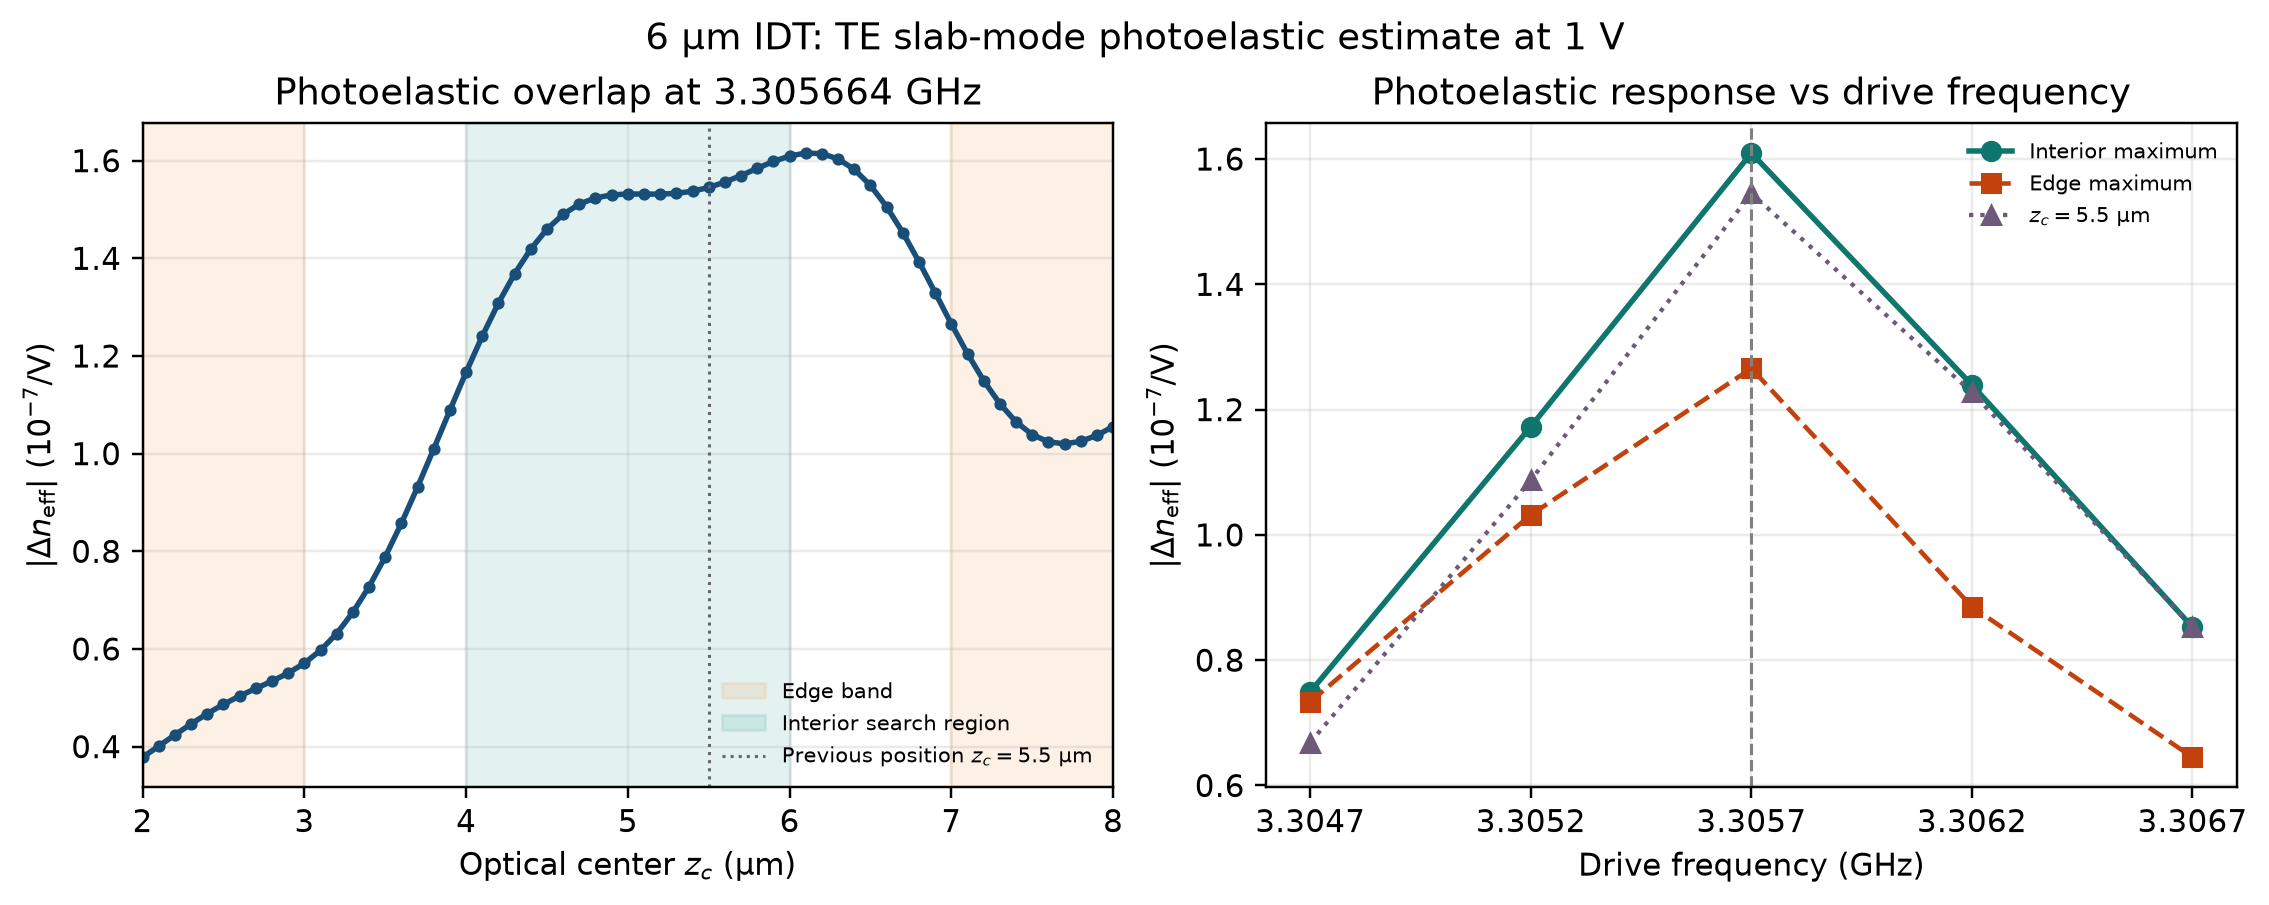
\includegraphics[width=\columnwidth]{images/drive_photoelastic_per_V.png}\caption{First-order photoelastic effective-index perturbation per terminal volt from the 100/50 nm 6 µm driven model using assumed TE slab-mode and Gaussian weighting. Left: spatial profile at 3.305664 GHz; shaded zones denote the chosen edge and interior bands. Right: interior maximum, edge maximum, and value at $z_c=5.5$ µm over the five-point frequency sweep. Actual optical eigenmode and moving-boundary terms are not included.}\label{fig:drive-pe}\end{figure}
The complete validation audit and clean data exports are provided in the accompanying data directory.
\section{Fabrication and experimental validation (pending)}
\textbf{No fabrication or measurements are reported in this draft.} The following fields are intentionally reserved for completion after the chip is fabricated and characterized. Do not replace these entries with simulated values.
\begin{table}[h]\centering\caption{Fabrication record to be completed.}\label{tab:fabrication}\begin{tabular}{@{}p{0.53\columnwidth}p{0.34\columnwidth}@{}}\toprule
Item & Status/value\\\midrule
Wafer orientation/cut & Pending\\
LN thickness (measured) & Pending\\
Electrode material/thickness & Pending\\
Lithographic aperture & Pending\\
Etch/release process & Pending\\
SEM/optical images & Pending\\
Fabrication yield & Pending\\\bottomrule\end{tabular}\end{table}
\begin{table}[h]\centering\caption{Experimental results to be added after measurement.}\label{tab:measurements}\begin{tabular}{@{}p{0.50\columnwidth}p{0.37\columnwidth}@{}}\toprule
Measurement & Result\\\midrule
RF resonance frequency & Pending\\
Loaded $Q$ / linewidth & Pending\\
$S_{11}$ / admittance response & Pending\\
Optical insertion loss & Pending\\
AO modulation response near 3.3 GHz & Pending\\
Drive voltage / RF power & Pending\\
Measured modulation efficiency & Pending\\
Device-to-device variation & Pending\\\bottomrule\end{tabular}\end{table}
\section{Conclusion}
We numerically swept the aperture of a suspended 3D TFLN IDT structure and evaluated a polarization-dependent photoelastic overlap proxy using exported eigenmode strain fields. On the baseline mesh, a 6 µm aperture has a target-band candidate at 3.304 GHz with an interior proxy of 39.54 J$^{-1/2}$. An initial mesh-refinement audit shows that the mode ordering and the 6-versus-10 µm aperture ranking are not yet stable. The 6 µm geometry remains a promising candidate near 3.3 GHz, but no mesh-converged optimum is established. Coupled-mode tracking and a mode-projected 1 V resonance are now available for one 6 µm model. Mass-normalized response, convergence of the driven projection and fitted linewidth across meshes, optical modulation analysis, and ultimately fabrication measurements remain necessary before claims about realized device performance.
\section*{Data and code availability}
The numerical data and analysis scripts are maintained with the project repository. A persistent public archive and version identifier should be added here before public release. COMSOL model files and raw solver exports are currently retained locally and are not included in the repository.
\section*{Author contributions} [To be completed.]
\section*{Funding} [To be completed.]
\section*{Competing interests} The authors declare [to be completed].
\begin{thebibliography}{9}
\bibitem{Cai2019} L. Cai, A. Mahmoud, and G. Piazza, ``Acousto-optical modulation of thin film lithium niobate waveguide devices,'' \emph{Photonics Research}, vol. 7, no. 9, pp. 1003--1013 (2019). doi: \href{https://doi.org/10.1364/PRJ.7.001003}{10.1364/PRJ.7.001003}.
\bibitem{Maity2019} S. Maity, M. Zhang, F. N. C. Wong, and M. Lon\v{c}ar, ``Microwave-to-optical conversion using lithium niobate thin-film acoustic resonators,'' \emph{Optica}, vol. 6, no. 12, pp. 1498--1505 (2019). doi: \href{https://doi.org/10.1364/OPTICA.6.001498}{10.1364/OPTICA.6.001498}.
\bibitem{Yu2021} Y. Yu, L. Wang, and X. Sun, ``Demonstration of on-chip gigahertz acousto-optic modulation at near-visible wavelengths,'' \emph{Nanophotonics}, vol. 10, no. 17, pp. 4323--4329 (2021). doi: \href{https://doi.org/10.1515/nanoph-2021-0330}{10.1515/nanoph-2021-0330}.
\bibitem{Chen2021} Z. Yu and X. Sun, ``Gigahertz acousto-optic modulation and frequency shifting on etchless lithium niobate integrated platform,'' \emph{ACS Photonics}, vol. 8, pp. 798--803 (2021). doi: \href{https://doi.org/10.1021/acsphotonics.0c01607}{10.1021/acsphotonics.0c01607}.
\end{thebibliography}
\end{document}
